\chapter{Requirement Analysis}
\label{chap:requirement-analysis}

\section{Stakeholder Analysis}
\label{section:stakeholder-analysis}
<TIP: List your stakeholders for your project here/>

Stakeholders are individuals, groups, or entities that
have an interest, concern, or stake in a particular project, decision,
organization, or system. These are individuals or groups who can affect or be
affected by the outcomes of your project.

\section{User Stories}
\label{section:user-stories}
<TIP: Write user stories for each of your stakeholders here./>

User stories are a technique used in agile software
development to capture and describe functional requirements from an end
user's perspective. They are a way of expressing software features or
functionality in a simple, non-technical language that can be easily understood
by both developers and stakeholders.

\section{Use Case Diagram}
\label{section:use-case-diagram}
<TIP: Write a use case diagram for your project here. Refer to an
article “What is a use case diagram?” by Lucidchart for help./>

\section{Use Case Model}
\label{section:use-case-model}
A use case is a detailed description of how a system
interacts with an external entity (such as a user or another system) to
accomplish a specific goal. Use cases provide a high-level view of the
functionality of a system and help in capturing and documenting its
requirements from the perspective of end users.

<TIP: Write use cases for your project here. Make sure to use the
appropriate type of use case for each scenario (brief, casual, and fully-dressed
use case)./>

\section{User Interface Design}
\label{section:user-interface-design}
<TIP: Put the initial design of your application here. You can
showcase a detailed design of a specific page or a sitemap of your application.
See an example below./>

\begin{figure}[h]
    \centering
    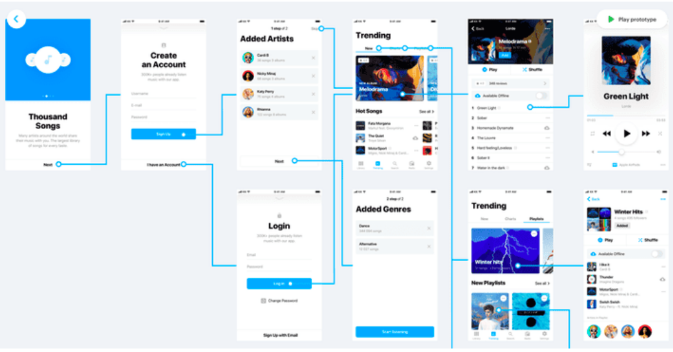
\includegraphics[width=0.8\textwidth]{examples/user-interface-design.png}
    \caption{User Interface Design}
\end{figure}